\documentclass{article}
\usepackage{graphicx} % Required for inserting images
\usepackage{amsmath}
\usepackage{tabularx}
\usepackage{subcaption}
\usepackage[
    colorlinks=true,  % Enables colored links
    linkcolor=blue,   % Color for links
    filecolor=blue,   % Color for file links
    urlcolor=blue,    % Color for URL links
    pdfborder={0 0 0}  % Removes the border around links
]{hyperref}
\usepackage{setspace}
\usepackage[a4paper, margin=1in]{geometry}

\title{My title}
\author{Amaury Maros}
\date{\today}

\onehalfspacing

\begin{document}

\maketitle

\tableofcontents

\newpage
\section{Section 1}

\subsection{Subsection 1}

\subsection{Subsection 2}

\section{Section 2}

\subsection{Subsection 2}

\begin{figure}[h!]
    \centering
    % Two figures side by side
    \begin{minipage}[b]{0.45\textwidth} % Adjust width for image A
        \centering
        \includegraphics[width=\textwidth,height=0.25\textheight,keepaspectratio]{figures/Figure1A.png} % Resize based on height
        \subcaption{}
        \label{fig:figure1A}
    \end{minipage}
    \hfill
    \begin{minipage}[b]{0.45\textwidth} % Adjust width for image B
        \centering
        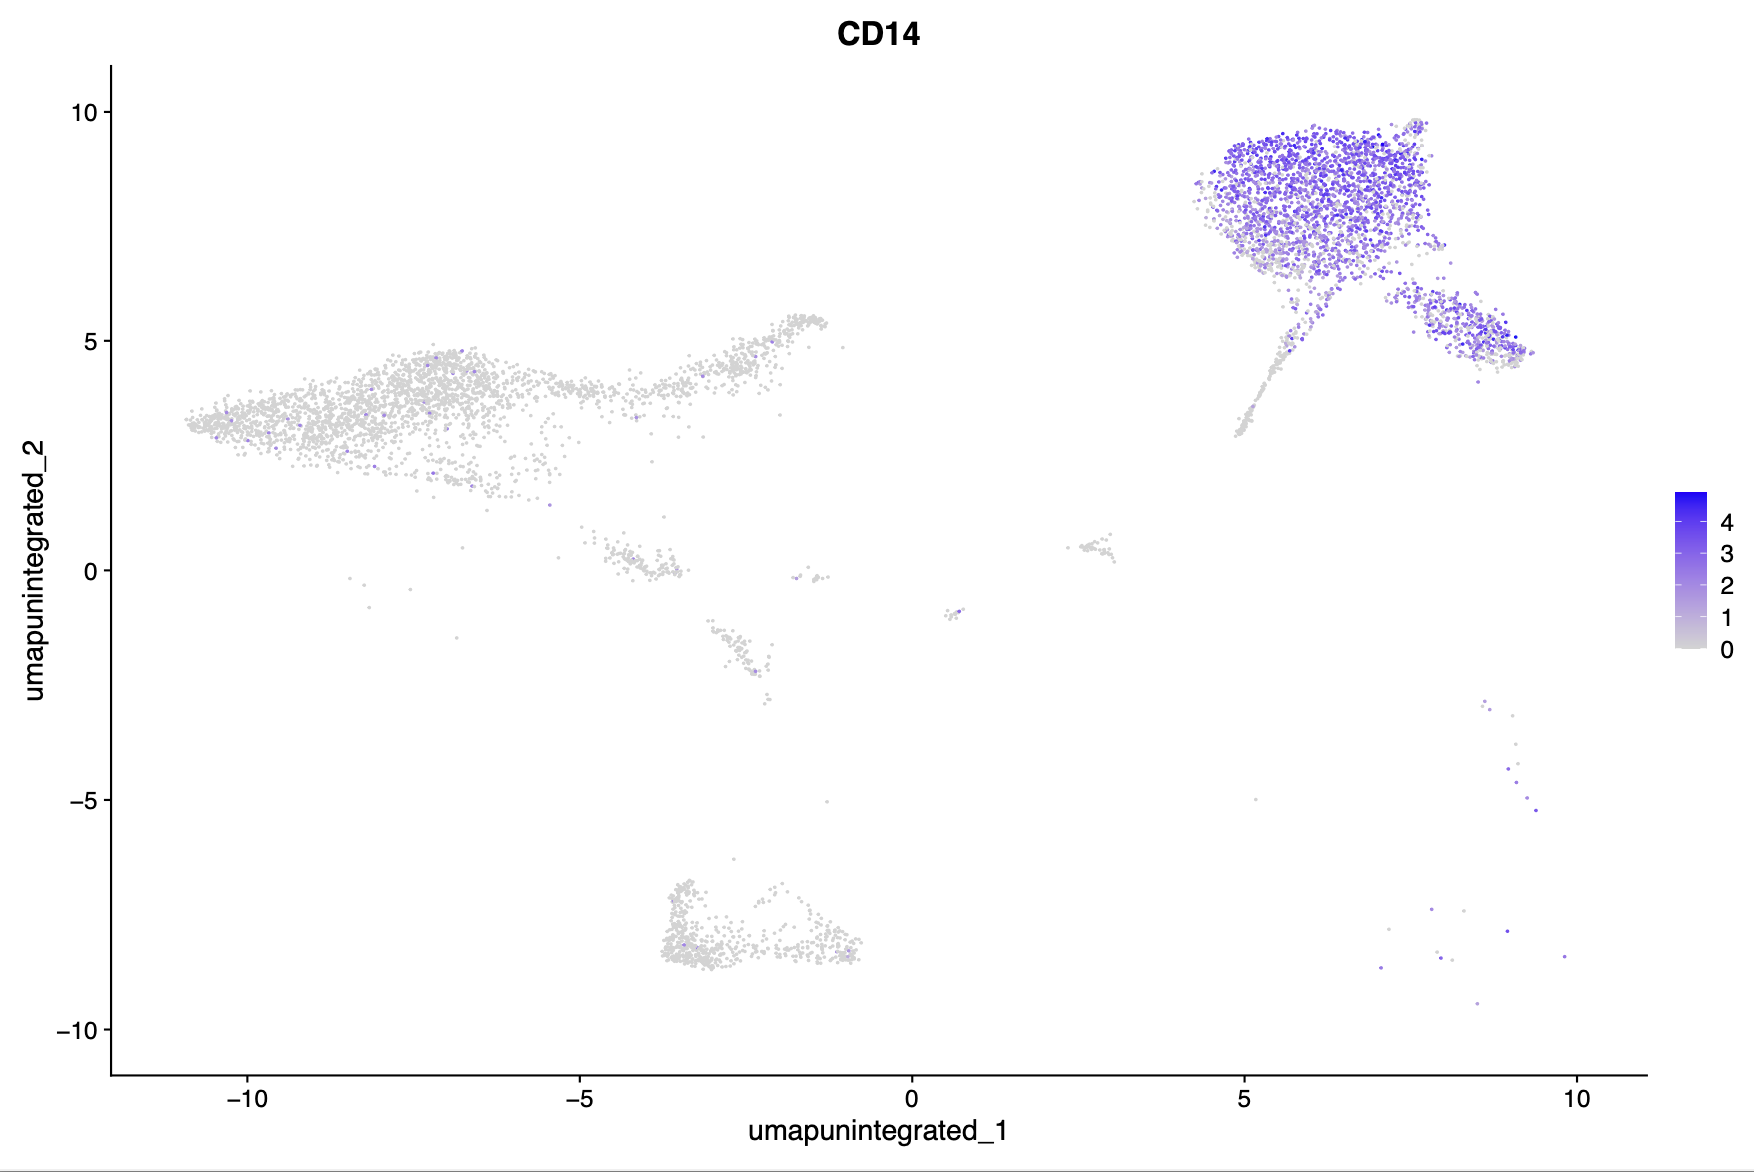
\includegraphics[width=\textwidth,height=0.25\textheight,keepaspectratio]{figures/Figure1B.png} % Resize based on height
        \subcaption{}
        \label{fig:figure1B}
    \end{minipage}
    
    % Figure C under
    \vskip 1em
    \begin{minipage}{\textwidth}
        \centering
        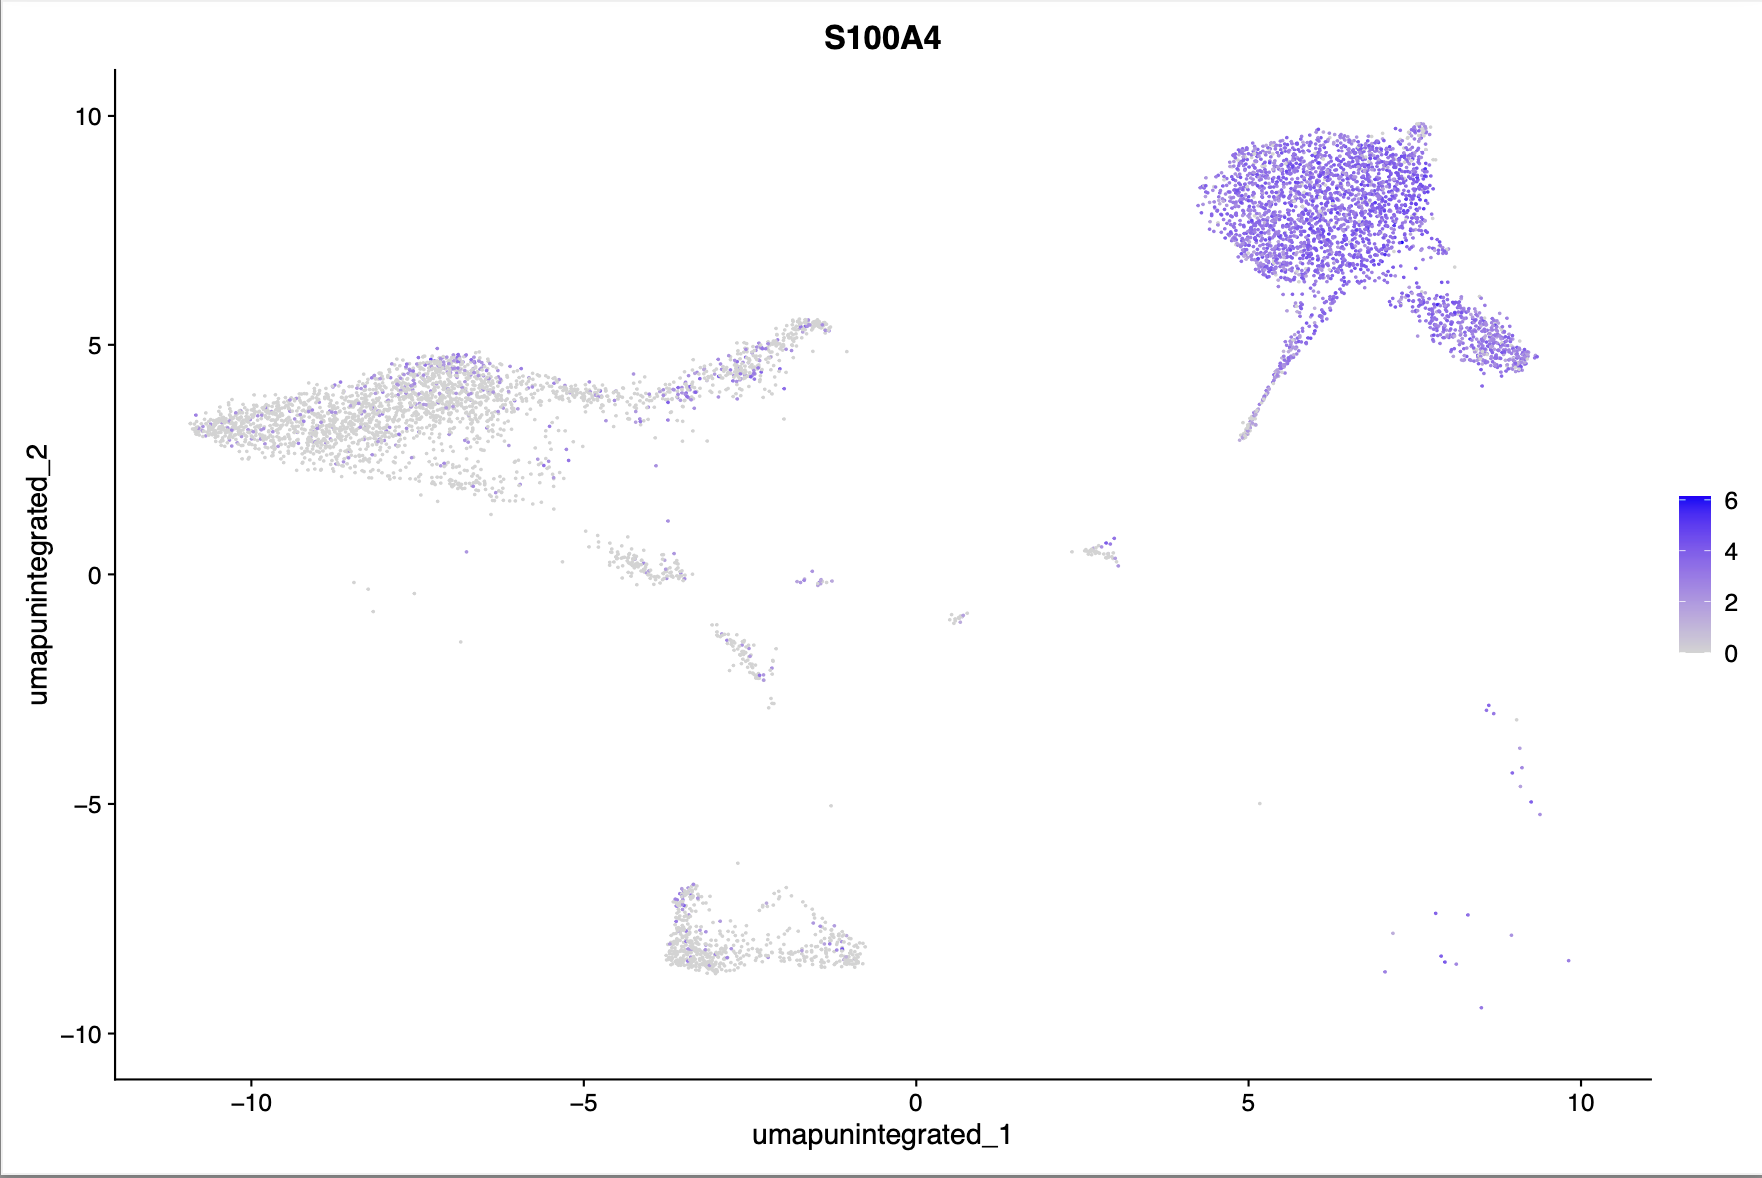
\includegraphics[width=0.45\textwidth,height=0.25\textheight,keepaspectratio]{figures/Figure1C.png} % Resize based on height
        \subcaption{}
        \label{fig:figure1C}
    \end{minipage}
    
    \captionsetup{justification=centering}
    \caption{Figure caption describing all subfigures (A, B, and C).}
\end{figure}



\section{Appendix}
\label{sec:appendix}


\begin{itemize}
    \item \textbf{Function}:  
    some text
    
    \item \textbf{Output}:  
    See Table~\ref{tab:my_table}
        
    \item \textbf{Contents}:  
    some text
\end{itemize}


\begin{table}[h!]
\centering
\begin{tabularx}{\textwidth}{|X|X|}
\hline
\textbf{Column 1} & \textbf{Column 2} \\ \hline
content 1.1 & content 2.1 \\ \hline
content 1.2 & content 2.2 \\ \hline

\end{tabularx}
\caption{Table caption}
\label{tab:my_table}
\end{table}

\end{document}
